\chapter{CMS Binary Chip}
\label{ac:cbc}

Prior to PhD research, the author carried out characterisation studies of the CMS Binary Chip (CBC) for his
MSc thesis. The CBC is the proposed 128 channel application specific integrated-circuit (ASIC) readout chip
for the silicon strip tracker sub-detector of CMS~\cite{JacobJA}. These studies were continued during the
beginning months of the PhD, as presented in the following sections.

\section{Introduction and previous studies}
\label{s:introduction_and_previous_studies}

Upgrades to the LHC over the coming years (Phase I) will lead to improvements in the operating parameters of
the LHC detailed in Section~\ref{s:Introduction}. By 2023, the luminosity delivered by the LHC is expected to
be $2\times10^{34}\mathrm{cm^{-2}s^{-1}}$. After 2023 (Phase 2), Long Shutdown 3 is planned to implement
further performance upgrades and will lead to a luminosity of $5\times10^{34}\mathrm{cm^{-2}s^{-1}}$.
The planned schedule of shutdowns and upgrades over the next decade can be seen
in Figure~\ref{fig:lhc_upgrades}.

The High Luminosity LHC (HL-LHC), as the machine will be known after Long Shutdown 3, will experience higher
collision rates. Therefore, there is a requirement for an upgraded CMS tracker in order to overcome the
problem of radiation damage suffered during previous years of data taking; to ensure it is capable of
withstanding the subsequent higher radiation levels;q and to allow the tracker to maintain performance with
the resulting 100-200 proton-proton interactions per bunch crossing~\cite{Mersi:2011jv}.

\begin{figure}[ht] %btp!]
   \centering
     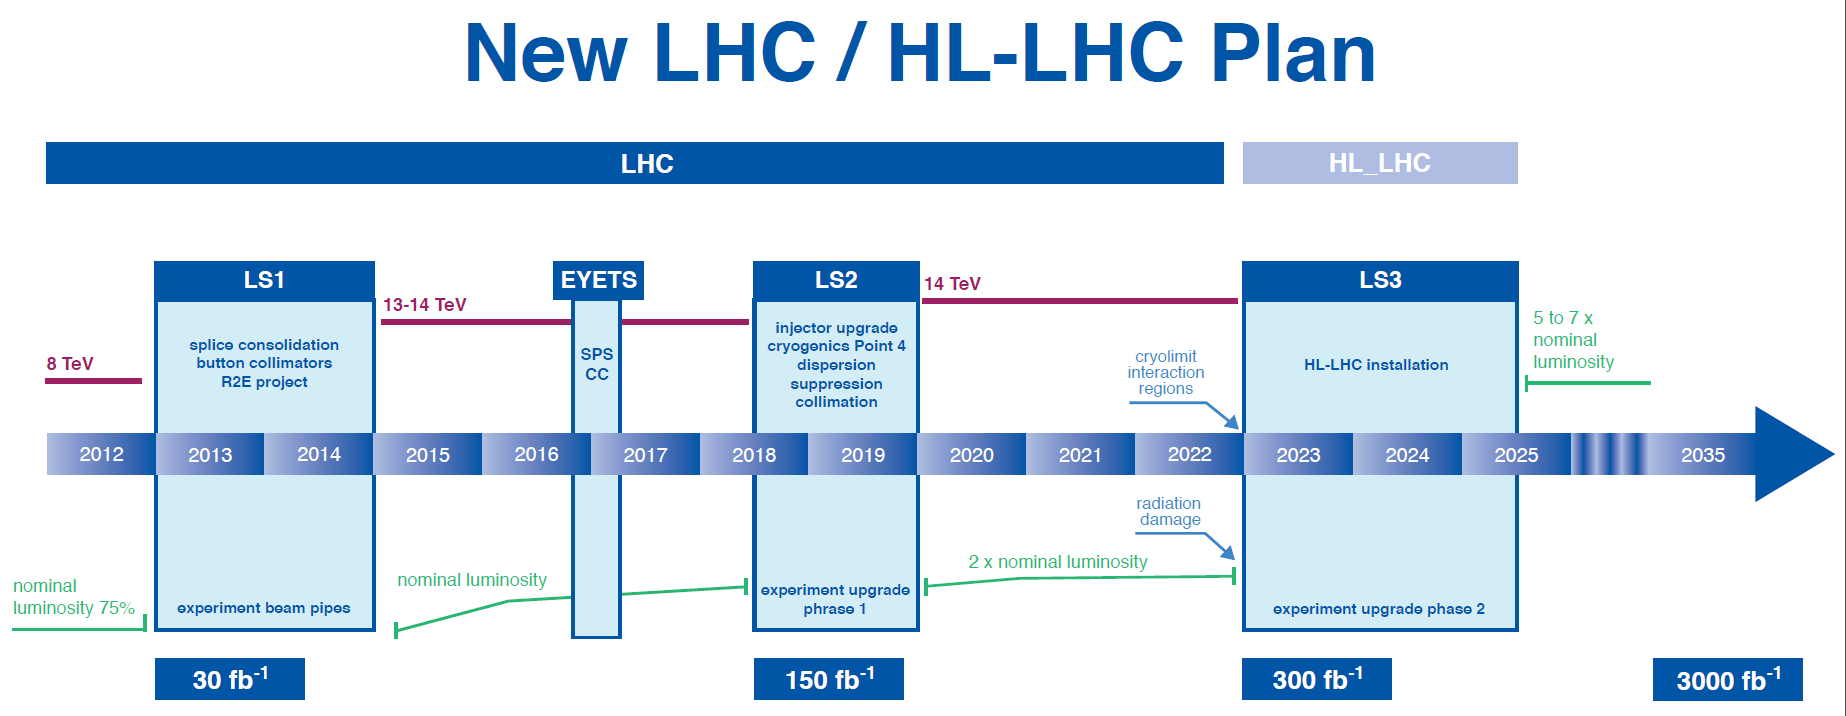
\includegraphics[width=0.8\textwidth]{Chapters/07_Appendices/07c_2_Images/newlhcplan}\hfill
     \caption{Schedule of LHC upgrades over the next decade.}
     \label{fig:lhc_upgrades}
\end{figure}

A description of the CBC is given in~\cite{JonesL}, and summarised together with a description of the
laboratory setup in~\cite{JacobJA}. In summary, the laboratory setup consisted of the CBC held on a CBC
carrier board, connected via an FPGA mezzanine card (FMC) to a field programmable gate array (FPGA) which was
connected to a controlling computer. The signal created in a connected silicon sensor would enter
the CBC through the analogue front end and a comparator digitises the signal to produce a binary output, a `1'
to indicate a `hit' or `0'. The CBC includes a setting to read out either `electrons' or `holes', and 24 of
the 128 channels were wire bonded out from the chip to allow signal to be injected if desired. TODO: GIVE
MORE CBC DESCRIPTION IF TIME ALLOWS %TODO: EXPAND ON THIS CBC DESCRIPTION A LITTLE IF TIME

\begin{figure}[ht] %btp!]
   \centering
     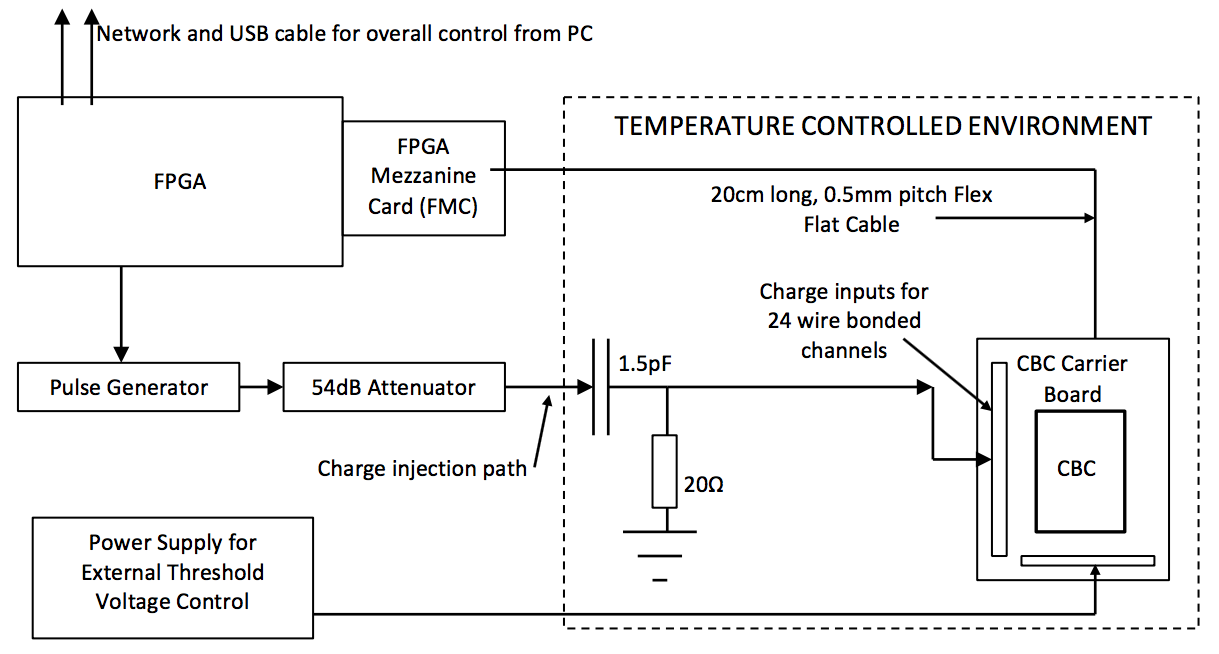
\includegraphics[width=0.8\textwidth]{Chapters/07_Appendices/07c_2_Images/lab_setup_schematic}\hfill
     \caption{Schematic of laboratory setup.}
     \label{fig:lab_setup_schematic}
\end{figure}

The introduction of the CBC to the CMS strip tracker will also lead to the provision of tracker data to the L1
trigger (tracker data is currently only used at HLT level, meaning L1 trigger decisions are made using only
muon chamber and calorimeter information). The design of the CBC is largely driven by this trigger
contribution requirement in order to maintain a practical L1 trigger rate in the high luminosity environment.
The upgraded strip tracker will also require a higher granularity in order to maintain low occupancy (a few
percent). Simultaneously, a low amount of tracker material should be maintained in order that particle
interactions with dead material are minimised, so that tracks with low \pt can be measured efficiently. The
increased number of channels will require the design power demand of the CBC to be lowered to a target
0.5~\mW/channel~\cite{JonesL,Ferguson:2012cg,Raymond:2012zz} compared to the current 2.7~\mW/channel of
the Analogue Pipeline Voltage 25 (APV25) tracker readout chip. This aim is accomplished in part by moving
from analogue to digital readout with the CBC.

Tests were carried out on the first CBC prototype, CBCv1, to verify its operation, to get information about
the behaviour of the analogue front-end, to test the response of the CBC to varying sizes of injected charges,
to measure the gain at a range of temperatures from -40~\degreeCelsius and 40~\degreeCelsius, and to measure
the channel-to-channel variation in pedestal voltage. The basic principle of the tests involved scanning
through the values of comparator threshold voltage, creating an s-curve', and evaluating the point at which
the mean output changed from zeros to ones or vice versa. These already documented tests were carried out only
on one chip, however. Continuation of that work, including some studies on a second CBCv1 chip, are outlined
below.

\section{Measuring signal noise using a capacitor}
\label{s:measuring_signal_noise_using_a_capacitor}

The noise in the test setup was investigated by attaching a capacitor to the CBC carrier board inputs for one
of the channels that was wire bonded to the CBC. At first, short wires were used (~1\cm in length) to
introduce a capacitance to the input signal. However, the capacitance of the board was too low (meaning the
capacitance of even very short wires was too high) for a useful measure of the noise in the signal to be
obtained from the resulting s-curves. Indeed, at no point during the scan of the channel offsets did the
comparator return all `1's or all `0's. After modifying the CBC carrier board to allow a capacitor to be
plugged directly into an input socket for the bonded channels, the tests were carried out with capacitors
ranging from 1~\pF to 10~\pF. The variation in the widths of these s-curves, a measure of the gaussian
distribution of noise in the signal, are shown in Figure~\ref{fig:noise_v_capacitance}. The plots for both
electrons and holes are similar and show no trends.

\begin{figure}[hbtp]
   \centering
     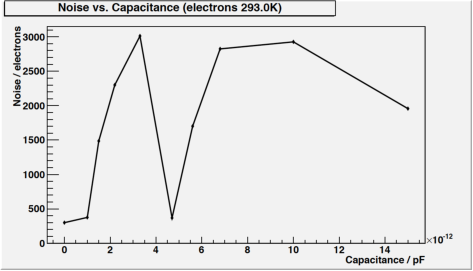
\includegraphics[width=0.5\textwidth]{Chapters/07_Appendices/07c_2_Images/noise_v_capacitance_ch_65_electrons}\hfill
     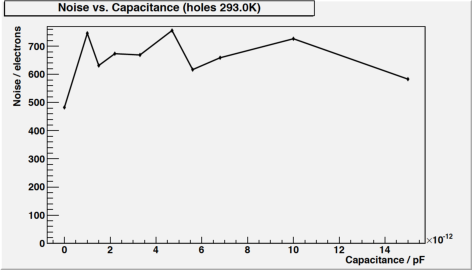
\includegraphics[width=0.5\textwidth]{Chapters/07_Appendices/07c_2_Images/noise_v_capacitance_ch_65_holes}\hfill
     \caption{Noise as a function of added capacitance for channel 65 in 'electrons' mode (left) and 'holes'
     mode (right).}
     \label{fig:noise_v_capacitance}
\end{figure}

The erratic variations over such small changes in capacitance may be explained by the fact that the noise
present in the test setup was showing levels of the order of thousands of electrons. The tests to study
the variation in noise as a function of added capacitance to an injection channel were therefore of little
use, due to the added noise now being so small compared to the noise in the test setup. After establishing
that the noise in the system was associated to the incoming pulse, additional grounding and shielding was
introduced in the form of copper tape, insulation between the connecting cables, placing the chip and it's
carrier board inside an aluminium box and injecting the pulse through a triaxial cable rather than a coaxial
cable. Unfortunately the latest results after all these modifications (Figure~\ref{fig:noise_all_channels})
show that although the noise on channels which are not connected to the pulse injection cable was reduced
to an acceptable level (about 200 electrons), the noise on the connected channel is still extremely high.
% Ferrite clamps on the connecting cable may improve the situation, but it remains to be discussed exactly
% what the next course of action will be.
The apparent limit of 200 electrons at the lower end of the scale is assumed to be due to the granularity of
the threshold voltage scans; using finer steps would have resulted in a smaller s-curve width, i.e. lower
noise.

\begin{figure}[hbtp]
   \centering
     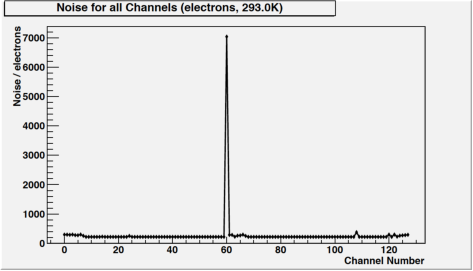
\includegraphics[width=0.5\textwidth]{Chapters/07_Appendices/07c_2_Images/noise_all_channels_60_connected_no_pulse_electrons}\hfill
     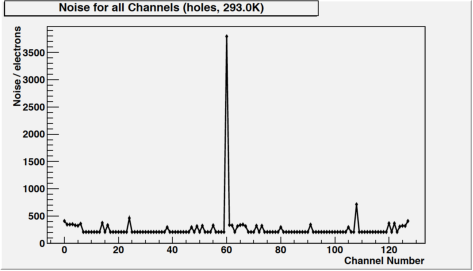
\includegraphics[width=0.5\textwidth]{Chapters/07_Appendices/07c_2_Images/noise_all_channels_60_connected_no_pulse_holes}
     \caption{Noise for all channels with injection cable connected to channel 60 but with no pulse injected,
     in 'electrons' mode (left) and 'holes' mode (right).}
     \label{fig:noise_all_channels}
\end{figure}


\section{Gain}
\label{s:gain}

The gain measurement for a second CBC was measured from the data obtained by varying the injected pulse
magnitude from the pulse generator to the CBC between 0.3~\fC and 4.8~\fC. Firstly, by varying the delay
between sending a pulse and taking a triggered data sample from the CBC, a picture can be built up of the
behaviour of the analogue front-end of the CBC. This will, in fact, give a measure of the voltage in the
postamplifier convoluted with any voltage offset in the comparator. Plots of the s-curve mid-point for the
range of delays (in steps of 1\ns) is shown for four injected sizes of injected charge in
Figure~\ref{subfig:scurve_midpoint_v_pg_delay_holes_20deg}.

The gain, defined as the mean ratio of the output signal to the input of a system. A plot of the difference
between the peak and the pedestal voltages as a function of injected charge can be produced
(Figure~\ref{subfig:scurve_midpoint_v_injected_charge_holes_20deg}), from which the gradient gives the gain of
the CBC at 20~\degreeCelsius in `holes' mode. This value was calculated as $31.7\pm1.1\mV/\fC$

\begin{figure}[hbtp]
	\centering
   	\subfloat[]{
   		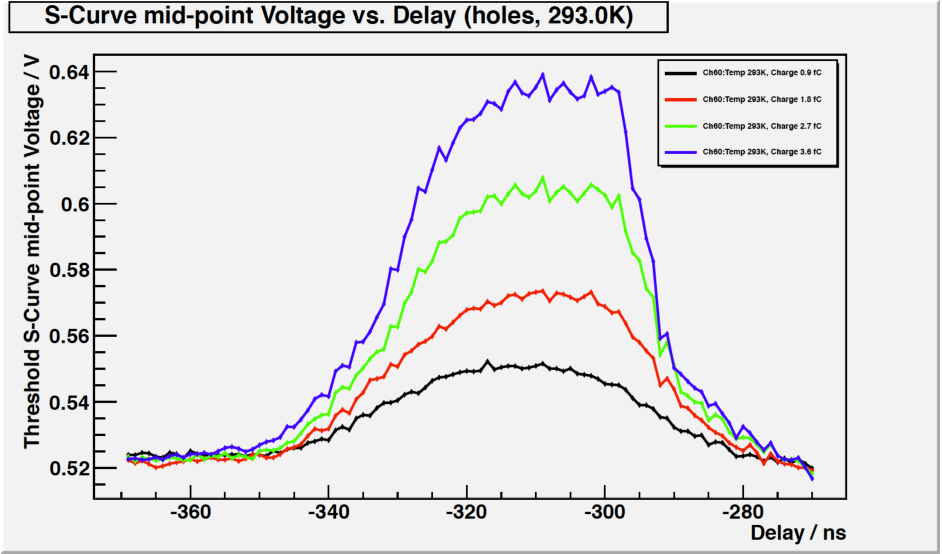
\includegraphics[width=0.5\textwidth]{Chapters/07_Appendices/07c_2_Images/scurve_midpoint_v_pg_delay_holes_20deg}
		\label{subfig:scurve_midpoint_v_pg_delay_holes_20deg}
		}
   	\subfloat[]{
   		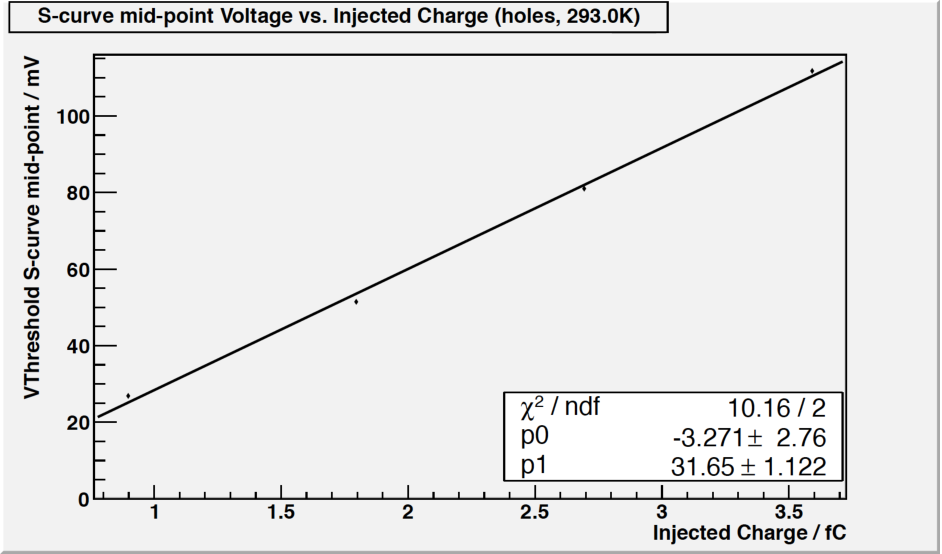
\includegraphics[width=0.5\textwidth]{Chapters/07_Appendices/07c_2_Images/scurve_midpoint_v_injected_charge_holes_20deg}
   		\label{subfig:scurve_midpoint_v_injected_charge_holes_20deg}
   	}
	\caption{S-curve mid-point (a) as a function of pulse generator delay and (b) as a function of injected
    charge in 'holes' mode at 20~$^{\circ}$C.}
    \label{fig:midpoint_v_delay_and_charge_holes_20deg}
\end{figure}


%    \begin{subfigure}[h]{0.5\textwidth}%[width=0.5\textwidth]
%    	 \centering
%    	 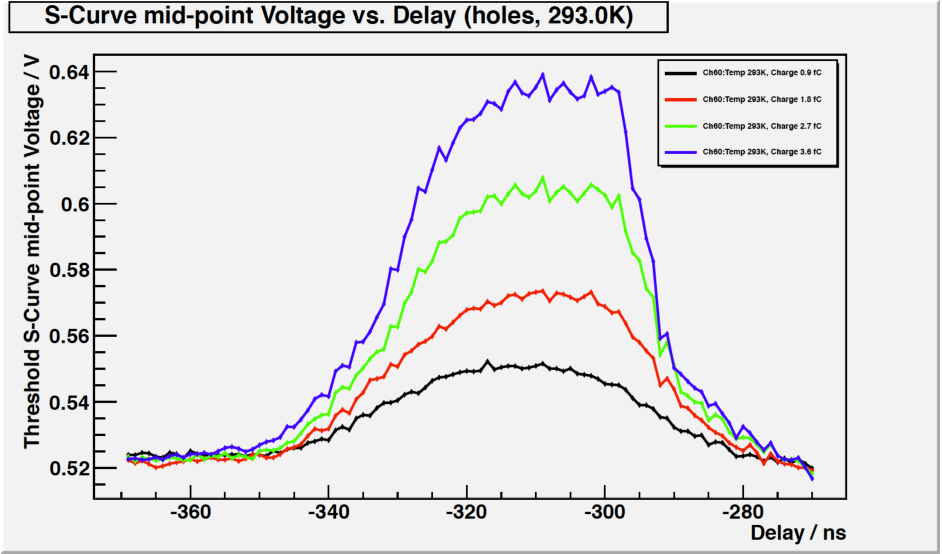
\includegraphics[width=\textwidth]{Chapters/07_Appendices/07c_2_Images/scurve_midpoint_v_pg_delay_holes_20deg}
%    	 \caption{}
%    	 \label{subfig:scurve_midpoint_v_pg_delay_holes_20deg}
%    \end{subfigure}
%    \begin{subfigure}[h]{0.5\textwidth} %[width=0.5\textwidth]
%    	 \centering
%    	 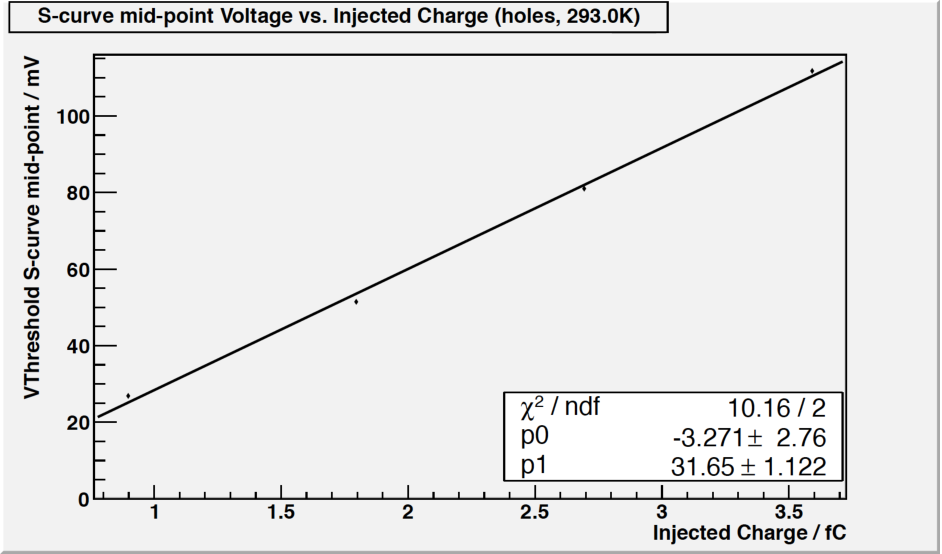
\includegraphics[width=\textwidth]{Chapters/07_Appendices/07c_2_Images/scurve_midpoint_v_injected_charge_holes_20deg}\hfill
%    	 \caption{}
%    	 \label{subfig:scurve_midpoint_v_injected_charge_holes_20deg}
%    \end{subfigure}
%      \caption{S-curve mid-point (a) as a function of pulse generator delay and (b) as a function of injected
%      charge in 'holes' mode at 20~$^{\circ}$C.}
%      \label{fig:midpoint_v_delay_and_charge_holes_20deg}
% \end{figure}

\section{Investigating change in Preamp Input Branch Bias Current}
\label{s:investigating_change_in_preamp_input_branch_bias_current}
The `Ipre1' bias generator register of the CBC governs the current in the input to the preamplifier in the
front-end of the chip. Following scans over the Ipre1 range for a range of temperatures from
-40~\degreeCelsius to 40~\degreeCelsius (Figure~\ref{fig:midpoint_v_ipre1}), it was noted that the effect of
modifying the current in the preamplifier input seems to flatten out after showing an initial decrease between
10\uA and 100\uA for 'electrons' mode, and after an initial increase between values of 10\uA to 50\uA for
`holes' mode. This is a small effect, unlikely to affect data taking, but it would be good to investigate if
future versions of the CBC exhibit similar behaviour.

\begin{figure}[hbtp]
   \centering
     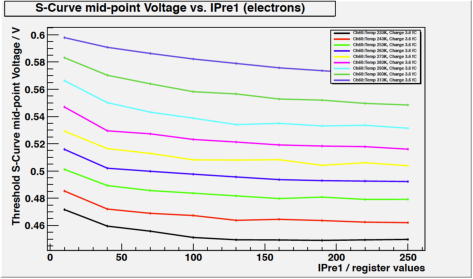
\includegraphics[width=0.5\textwidth]{Chapters/07_Appendices/07c_2_Images/scurve_midpoint_v_ipre1_electrons}\hfill
     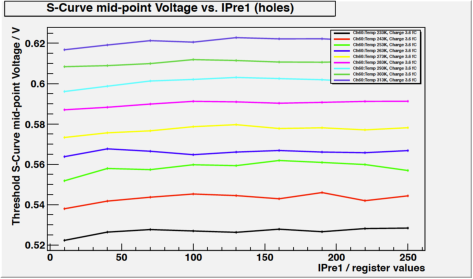
\includegraphics[width=0.5\textwidth]{Chapters/07_Appendices/07c_2_Images/scurve_midpoint_v_ipre1_holes}
     \caption{Variation in s-curve mid-point over range of Ipre1 register values for temperatures from
     -40~$^{\circ}$C to 40~$^{\circ}$C.}
     \label{fig:midpoint_v_ipre1}
\end{figure}

\section{Summary}
\label{s:summary}
This chapter has presented a short report based on the continuation of work from the author's MSc
investigation the CBC. Attempts were made to characterise the noise in the CBC using additional capacitors,
but these showed that the noise levels in the test setup were excessively high. Attempts were made to reduce
this to below the CBC front-end design specification of 1000 electrons. However, the impact of the actions
taken were enough only to reduce the noise on CBC channels that are not wire-bonded to approximately 200
electrons, while the noise present in a bonded channel connected to the pulse generator was still several
thousand electrons.

The gain of a second CBC was measured in `holes' mode at 20~\degreeCelsius as $31.7\pm1.1\mV/\fC$, which is in
agreement with typical values of readout chips at silicon detectors of between approximately 15\mV/\fC and
40\mV/\fC~\cite{Kaplon:2001jh}. The bias generator regulating the current input to the preamplifier was
investigated over its register range at temperatures from -40~\degreeCelsius to 40~\degreeCelsius. It was
found that in the region up to 100\uA, the comparator voltage decreased in `electrons' mode, and up to 50\uA
increased for `holes' mode.

Following the work in~\cite{JacobJA} and that presented here, testing has continued on a newer 254-channel
version of the chip (CBC2), with triggering capability on-board to contribute to the Level 1 trigger and
designed to be bump-bonded as opposed to wire bonded~\cite{Klein:1628930,Abbaneo:1452189}.
Prototypes of the modules that will carry the CBCs when installed in the CMS detector have also been produced
and tested. The subsequent CBC3 is currently in the design and is scheduled to be available for testing in
approximately May 2016, with an `insurance' CBC4 scheduled, if necessary, for testing to begin with the final
version in 2018.
